\documentclass{article}
\usepackage{amssymb}
\usepackage[utf8]{inputenc}
\usepackage{geometry}
\usepackage{mathtools}
\usepackage{verbatim}

\geometry{letterpaper, portrait, margin=1in}

\title{CS325 - Project 4}
\author{Group \#6 \\ William Jernigan, Alexander Merrill, Sean Rettig}
\date{\today}

\begin{document}

\maketitle

\part*{Problem 1: mmmm ... tofu}
\section*{Mathematical Representation}
\paragraph*{Variables:\\}
$u_f$ = working day flavored blocks of tofu\\
$m_f$ = working day flavored bags of edamame\\
$p_f$ = working day flavored blocks of tempeh\\
$u_o$ = overtime flavored blocks of tofu\\
$m_o$ = overtime flavored bags of edamame\\
$p_o$ = overtime flavored blocks of tempeh\\
$u_p$ = plain blocks of tofu\\
$m_p$ = plain bags of edamame\\
$p_p$ = plain blocks of tempeh\\

\paragraph*{Objective:}
max \{$4u_p + 12u_f + 7u_o + 8m_p + 14m_f + 11m_o + 4p_p + 13p_f + 9p_o$\}
\paragraph*{Set of Constraints:\\}
$u_f + u_o + u_p \leq 480$\\ %tofu <= 480
$m_f + m_o + m_p \leq 400$\\ %edamame <= 400
$p_f + p_o + p_p \leq 230$\\ %tempeh <= 230
$u_f + m_f + p_f \leq 420$\\ %flavored on reg. time <= 420
$u_o + m_o + p_o \leq 250$\\ %flavored on overtime <= 250
$-u_f \leq 0$\\
$-m_f \leq 0$\\
$-p_f \leq 0$\\
$-u_o \leq 0$\\
$-m_o \leq 0$\\
$-p_o \leq 0$\\
$-u_p \leq 0$\\
$-m_p \leq 0$\\
$-p_p \leq 0$\\


\section*{Matrix Representation}

\[
\begin{array}{cccc}
\left[ \begin{array}{ccccccccc}
1 & 0 & 0 & 1 & 0 & 0 & 1 & 0 & 0\\
0 & 1 & 0 & 0 & 1 & 0 & 0 & 1 & 0\\
0 & 0 & 1 & 0 & 0 & 1 & 0 & 0 & 1\\
1 & 1 & 1 & 0 & 0 & 0 & 0 & 0 & 0\\
0 & 0 & 0 & 1 & 1 & 1 & 0 & 0 & 0\\
-1 & 0 & 0 & 0 & 0 & 0 & 0 & 0 & 0\\
0 & -1 & 0 & 0 & 0 & 0 & 0 & 0 & 0\\
0 & 0 & -1 & 0 & 0 & 0 & 0 & 0 & 0\\
0 & 0 & 0 & -1 & 0 & 0 & 0 & 0 & 0\\
0 & 0 & 0 & 0 & -1 & 0 & 0 & 0 & 0\\
0 & 0 & 0 & 0 & 0 & -1 & 0 & 0 & 0\\
0 & 0 & 0 & 0 & 0 & 0 & -1 & 0 & 0\\
0 & 0 & 0 & 0 & 0 & 0 & 0 & -1 & 0\\
0 & 0 & 0 & 0 & 0 & 0 & 0 & 0 & -1\\
\end{array} \right]
&
\left[ \begin{array}{c}
u_f\\
m_f\\
p_f\\
u_o\\
m_o\\
p_o\\
u_p\\
m_p\\
p_p 
\end{array} \right]
&
\leq
&
\left[ \begin{array}{c}
480\\
400\\
230\\
420\\
250\\
0\\
0\\
0\\
0\\
0\\
0\\
0\\
0\\
0 \end{array} \right]
\\
"A" & X^T & & "b"
\end{array}
\]

\section*{Optimal Solution}
The maximum profit that can be made is \$10,610 with the following plan:\\
tofu plain = 60\\
tofu flavored on regular time = 420\\
tofu flavored on overtime = 0\\
edamame plain = 380\\
edamame flavored on regular time = 0\\
edamame flavored on overtime = 20\\
tempeh plain = 0\\
tempeh flavored on regular time = 0\\
tempeh flavored on overtime = 230\\

\section*{Environment Used to Solve}
GUSEK is an open source Windows GUI which provides a SciTE editor for describing LPs and solves them with GLPK, a standalone tool usable in command line.

\section*{Code}
\verbatiminput{p4_prob1.lp}

\pagebreak


\part*{Problem 2: least squares isn't good enough for me}
\section*{Linear Program for General Problem}
\paragraph*{Objective:}
min t

\paragraph*{Subject to:\\}
$-t + ax_i + by_i - c \leq 0$ for $1 \leq i \leq n$\\
$t + ax_i + by_i - c \leq 0$ for $1 \leq i \leq n$\\
$t \geq 0$\\

\section*{Best Solution for Specific Problem}
\paragraph*{Objective:}
min t

\paragraph*{Subject to:\\}
$t - a1 - b3 + c \leq 0$\\
$-t + a + 3b - c \leq 0$\\
$t + a + 3b - c \leq 0$\\
$-t + 2a + 5b - c \leq 0$\\
$t + 2a + 5b - c \leq 0$\\
$-t + 3a + 7b - c \leq 0$\\
$t + 3a + 7b - c \leq 0$\\
$-t + 5a + 11b - c \leq 0$\\
$t + 5a + 11b - c \leq 0$\\
$-t + 7a + 14b - c \leq 0$\\
$t + 7a + 14b - c \leq 0$\\
$-t + 8a + 15b - c \leq 0$\\
$t + 8a + 15b - c \leq 0$\\
$-t + 10a + 19b - c \leq 0$\\
$t + 10a + 19b - c \leq 0$\\
$-t \leq 0$\\


\section*{Plot and Solution}
\centerline{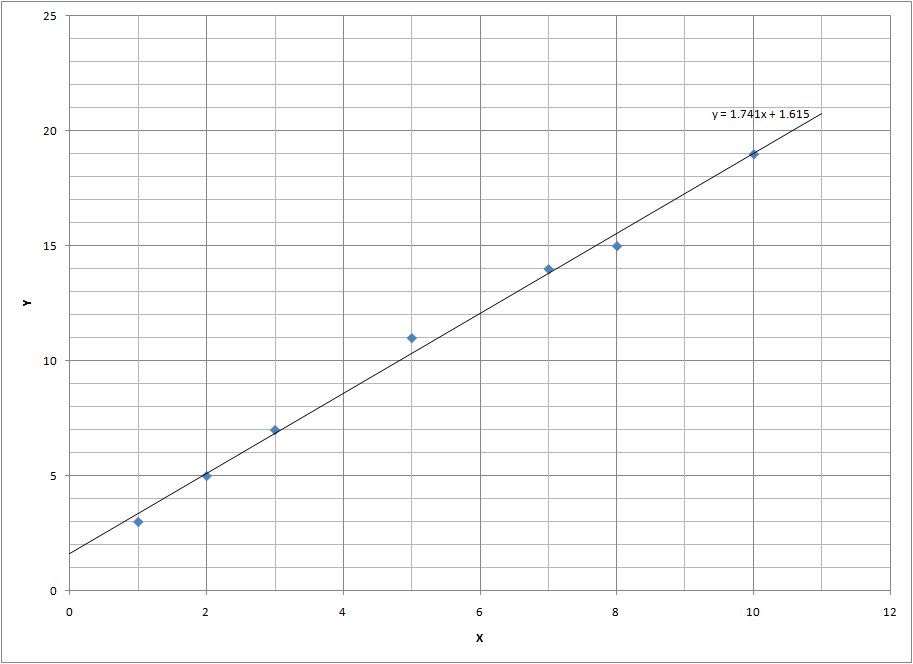
\includegraphics[width=0.75\textwidth]{plot.png}}

\section*{Code}
\verbatiminput{p4_prob2.lp}

\section{Work Shown}
Attached are copies of our work and scratch paper.

\end{document}
